\documentclass{beamer}
\usepackage[T2A]{fontenc}
\usepackage[utf8]{inputenc}
\usepackage[russian, english]{babel}
\usepackage{amssymb, amsfonts, amsmath, mathtext, cite, enumerate, float, indentfirst, graphicx, epstopdf, mathtools, color}

% Фикс ошибки с hyperref на linux
\hypersetup{unicode=true}

\usetheme{Warsaw}
\usecolortheme{beaver}

% Пытался настроить отображение номера слайда
\makeatletter
\defbeamertemplate*{footline}{my theme}{
    \leavevmode
    \hbox{
    \begin{beamercolorbox}[wd = \paperwidth, ht = 5ex, dp = 4ex, right]{}
        \insertframenumber{} / \inserttotalframenumber\hspace*{5ex}
    \end{beamercolorbox}}
}
\makeatother

% Убрать нижнюю панель навигации
\setbeamertemplate{navigation symbols}{}

% Убрать верхнюю панель навигации section/subsection 
\setbeamertemplate{headline}{}

% Цвет циферок для ссылок
\setbeamercolor{footnote mark}{fg = red}

% Вернуть нумерацию фигур
\setbeamertemplate{caption}[numbered]

\DeclarePairedDelimiter\bra{\langle}{\rvert}
\DeclarePairedDelimiter\ket{\lvert}{\rangle}

\begin{document}

%% -TITLE-
\title{Quantum Machine Learning: overview}
\author{M. E. Lebedev}
\date{(?) Apr. 2017 \\ Saint-Petersburg, IFMO}
%% -END-

%% -SLIDE-
\begin{frame}
\maketitle
\end{frame}
%% -END-

%% -SLIDE-
\begin{frame}
\frametitle{Quantum information approach}

{\bf Qbit} (quantum bit) is a {\bf superposition} state: $\ket{\psi} = \alpha \ket{0} + \beta \ket{1}$,
where $\ket{0}$, $\ket{1}$ (logical $0$, $1$) are two orthogonal states in Hilbert space for some two-level quantum system.

\medskip

$\alpha, \beta \in \mathbb{C}$, $|\alpha|^2$, $|\beta|^2$ --- probabilities to find qbit in the state $\ket{0}$ or $\ket{1}$ correspondingly.

\medskip

{\bf Normalization}: $|\alpha|^2 + |\beta|^2 = 1$.

\medskip

{\bf Physical realization}:
\begin{itemize}
\item Electrons in quantum dots: $\ket{0} = \ket{\uparrow}$, $\ket{1} = \ket{\downarrow}$.
\item Photon polarization: $\ket{0} = \ket{\updownarrow}$, $\ket{1} = \ket{\leftrightarrow}$.
\item Two level atomic system: $\ket{0} = \textrm{Ground state}$, $\ket{1} = \textrm{Excited state}$.
\end{itemize}

\end{frame}
%% -END-

%% -SLIDE-
\begin{frame}
\frametitle{Quantum excellence}

\begin{columns}
\begin{column}{0.5\textwidth}
\begin{center}
Classical computer
\end{center}
\end{column}

\begin{column}{0.5\textwidth}
\begin{center}
Qunatum computer
\end{center}
\end{column}
\end{columns}

\begin{columns}
\begin{column}{0.5\textwidth}

\begin{center}
$L$ {\bf bits} --- $1$ state:
$$\underbrace{0010101 \dots 011}_\text{$L$}$$
\end{center}

\end{column}
\begin{column}{0.5\textwidth}

\begin{center}
$L$ {\bf qbits} --- superposition of $2^L$ states
$$\underbrace{a_1 \ket{\dots} + a_2 \ket{\dots} + \dots + a_{2^L} \ket{\dots}}_\text{$2^L$}$$

\color{red}{$2^L$ complex amplitudes!}
\end{center}

\end{column}
\end{columns}

\vspace{1cm}

We can control quantum state: operators act in a $2^L$ - dimentional Hilbert space.
\end{frame}
%% -END-

%% -SLIDE-
\begin{frame}
\frametitle{Quantum gates}
Dirac notation: $\ket{0} = (1, 0)^T$, $\ket{1} = (0, 1)^T$.

\medskip

A, B -- two qbits, $\ket{0_A 0_B} = \ket{0_A} \otimes \ket{0_B} = (1, 0, 0, 0)^T$.

\begin{figure}
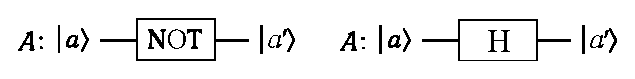
\includegraphics[width=0.8\textwidth]{pic/not_and_H.eps}
\end{figure}

$NOT = \begin{pmatrix} 0 & 1 \\ 1 & 0 \end{pmatrix}$, $H = \dfrac{1}{\sqrt{2}} \begin{pmatrix} 1 & 1 \\ 1 & -1 \end{pmatrix}$.

\begin{figure}
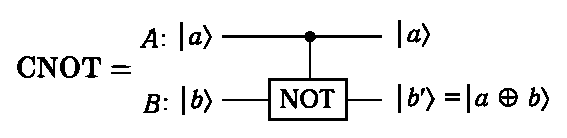
\includegraphics[width=0.7\textwidth]{pic/cnot.eps}
\end{figure}

$CNOT = \begin{pmatrix}
1 & 0 & 0 & 0 \\
0 & 1 & 0 & 0 \\
0 & 0 & 0 & 1 \\
0 & 0 & 1 & 0
\end{pmatrix}$, and many other different gates.

\end{frame}
%% -END-

%% -SLIDE-
\begin{frame}
\frametitle{Demonstration: Deutsch–Jozsa algorithm}
Functions $f_i$ act on a binary variable $x = 0,1$:

\medskip

$f_1(x) = 0$, $f_2(x) = 1$, $f_3(x) = x$, $f_4(x) = \bar{x}$.

\medskip

{\bf Task}: determine the type of $f_i$.

\medskip

Classical case: {\bf $2$} evaluation of $f$: $f(0)$, $f(1)$.

Quantum case: \underline{only $1$ operation}!

\begin{figure}
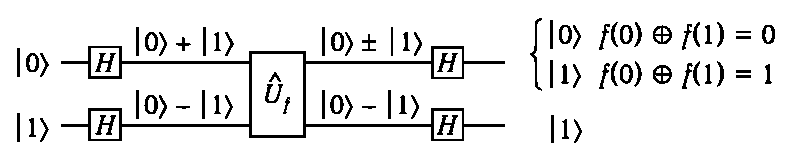
\includegraphics[width=0.9\textwidth]{pic/jozsa.eps}
\end{figure}

$$\hat{U}_f: \ket{x} \otimes \ket{y} \Rightarrow \ket{x} \otimes \ket{y \oplus f(x)}$$

\end{frame}
%% -END-


%% -SLIDE-
\begin{frame}
\frametitle{Grover's algorithm}

Boolean fucntion $f$ acts on $L$ -- dimensional boolean variables: $f: \{0, 1\}^L \to \{0, 1\}$.

\medskip

{\bf Task}: find a solution $x$, $f(x) = 1$.

\medskip

Classical case: $O(N)$ operations, $N = 2^L$.

\medskip 

Quantum case: \underline{$O(\sqrt{N})$ operations}!

\medskip

Usage of the Grover's algorithm:
\begin{itemize}
\item
\item
\item
\end{itemize}

\end{frame}
%% -END-


%% -SLIDE-
\begin{frame}
\frametitle{QML: current state of art}
\begin{figure}
\center{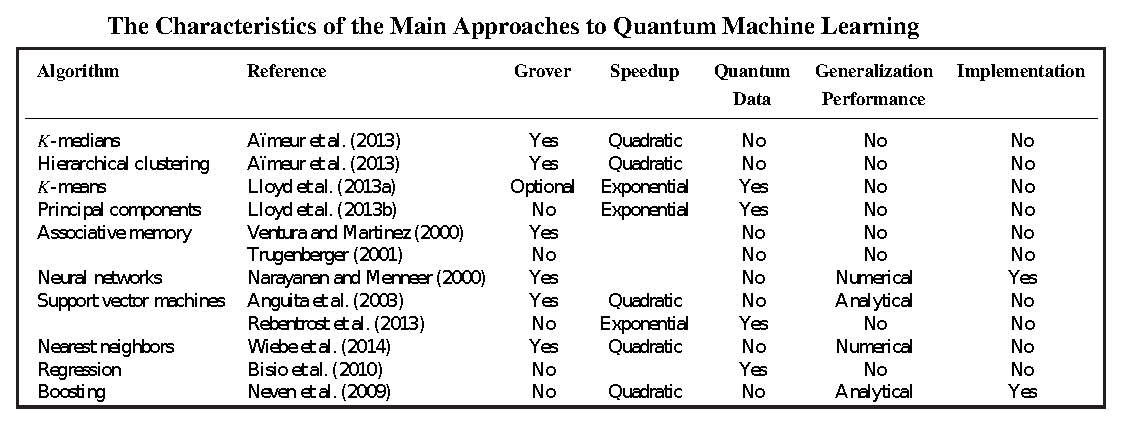
\includegraphics[width=1\textwidth]{pic/table.eps}}
\caption{Main Approaches to Quantum ML problem and related tasks\footnotemark[1]}
\end{figure}

\footnotetext[1]{\footnotesize{Peter Wittek, Quantum Machine Learning, Academic Press is an imprint of Elsevier, 2014}}
\end{frame}
%% -END-

%% -SLIDE-
\begin{frame}
\frametitle{Quantum annealing}
\end{frame}
%% -END-


%% -SLIDE-
\begin{frame}
\begin{center}
Thank for your attention!
\end{center}
\end{frame}
%% -END-

\end{document}